% !TeX spellcheck = ru_RU
% !TEX root = vkr.tex

\section{Архитектура решения}

\subsection{Детали реализации SpMSpV}

На платформе .NET существует поддержка параллельных вычислений с использованием асинхронных (т.~e не блокирующих выполнение других процессов) выражений \texttt{tasks}. Они позволяют разбить работу программы на небольшие подзадачи и запустить их параллельно на доступных вычислительных ядрах.

Так как эффективность параллельной версии алгоритма, главным образом, зависит от количества используемых потоков, для векторно-матричных операций были добавлены параметры \texttt{level} --- для сложения и \texttt{multiLevel}, \texttt{addLevel} --- для умножения. Эти аргументы представляют собой \textit{уровни распараллеливания}; к примеру, для ненулевого \texttt{level} функции \texttt{vectorAddition} (листинг. \ref{lst:add}) формируются две задачи, исполняемые параллельно,  для ненулевого \texttt{level -- 1} формируются ещё две подзадачи и т.~д.

\begin{lstlisting}[style=fsharp, caption={Часть функции сложения векторов, отвечающая за параллельную составляющую векторной операции.}, label={lst:add},  frame=single, firstnumber=33]
| BinTree.Node (x, y), BinTree.Node (z, w) ->
    if parallelLevel = 0u then
        let left = treesAddition 0u x z
        let right = treesAddition 0u y w

        if left = BinTree.None && right = BinTree.None then
            BinTree.None
        else
            BinTree.Node(left, right)
    else
        let tasks =
            [| async { return treesAddition (parallelLevel - 1u) x z }; 
            async { return treesAddition (parallelLevel - 1u) y w } |]

        let results = tasks |> Async.Parallel |> Async.RunSynchronously
\end{lstlisting}

\newpage

Аналогично сложению используются \texttt{multiLevel}, \texttt{addLevel} в функции \texttt{multi\-plication}, однако в процессе формируются четыре подзадачи вместо двух (листинг. \ref{lst:multi}). Это различие обусловлено строением вектора и матрицы: узлы дерева, представляющего вектор, имеют ровно два потомка, а узлы дерева, представляющие матрицу --- четыре. Примерная визуализация распределения задач между узлами вектора при сложении представлена на рис. \ref{fig:tree}, а последовательность выполнения операции --- на рис. \ref{fig:uml}.

\begin{lstlisting}[style=fsharp, caption={Часть функции умножения вектора и матрицы, отвечающая за параллельную составляющую векторно-матричной операции.}, label={lst:multi},  frame=single, firstnumber=93]
else
    let multiTasks =
       [| async { return Vector(multiTrees (parallelLevel - 1u) left first,
                  vector.Length) }
          async { return Vector(multiTrees (parallelLevel - 1u) right third,
                  vector.Length) }
          async { return Vector(multiTrees (parallelLevel - 1u) left second,
                  vector.Length) }
          async { return Vector(multiTrees (parallelLevel - 1u) right fourth,
                  vector.Length) } |]

    let multiResults = multiTasks |> Async.Parallel |> Async.RunSynchronously

    let leftTree1 = multiResults[0]
    let leftTree2 = multiResults[1]
    let rightTree1 = multiResults[2]
    let rightTree2 = multiResults[3]

    let addTasks =
       [| async { return (vectorAddition addLevel plusOperation
                  leftTree1 leftTree2).Storage }
          async { return (vectorAddition addLevel plusOperation
                  rightTree1 rightTree2).Storage } |]

    let addResults = addTasks |> Async.Parallel |> Async.RunSynchronously

\end{lstlisting}

\begin{figure}
    \centering
    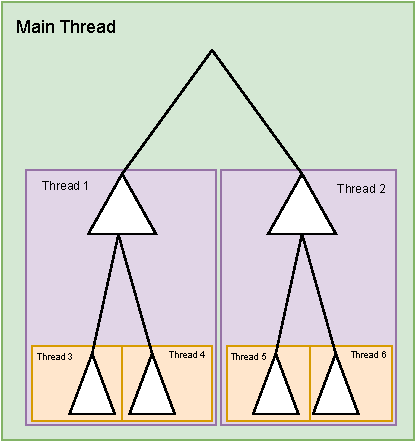
\includegraphics[width=0.6\textwidth]{QuadTree.pdf}
    \caption{Распределение потоков между узлами дерева, представляющего разреженный вектор, при сложении\\}
    \label{fig:tree}
    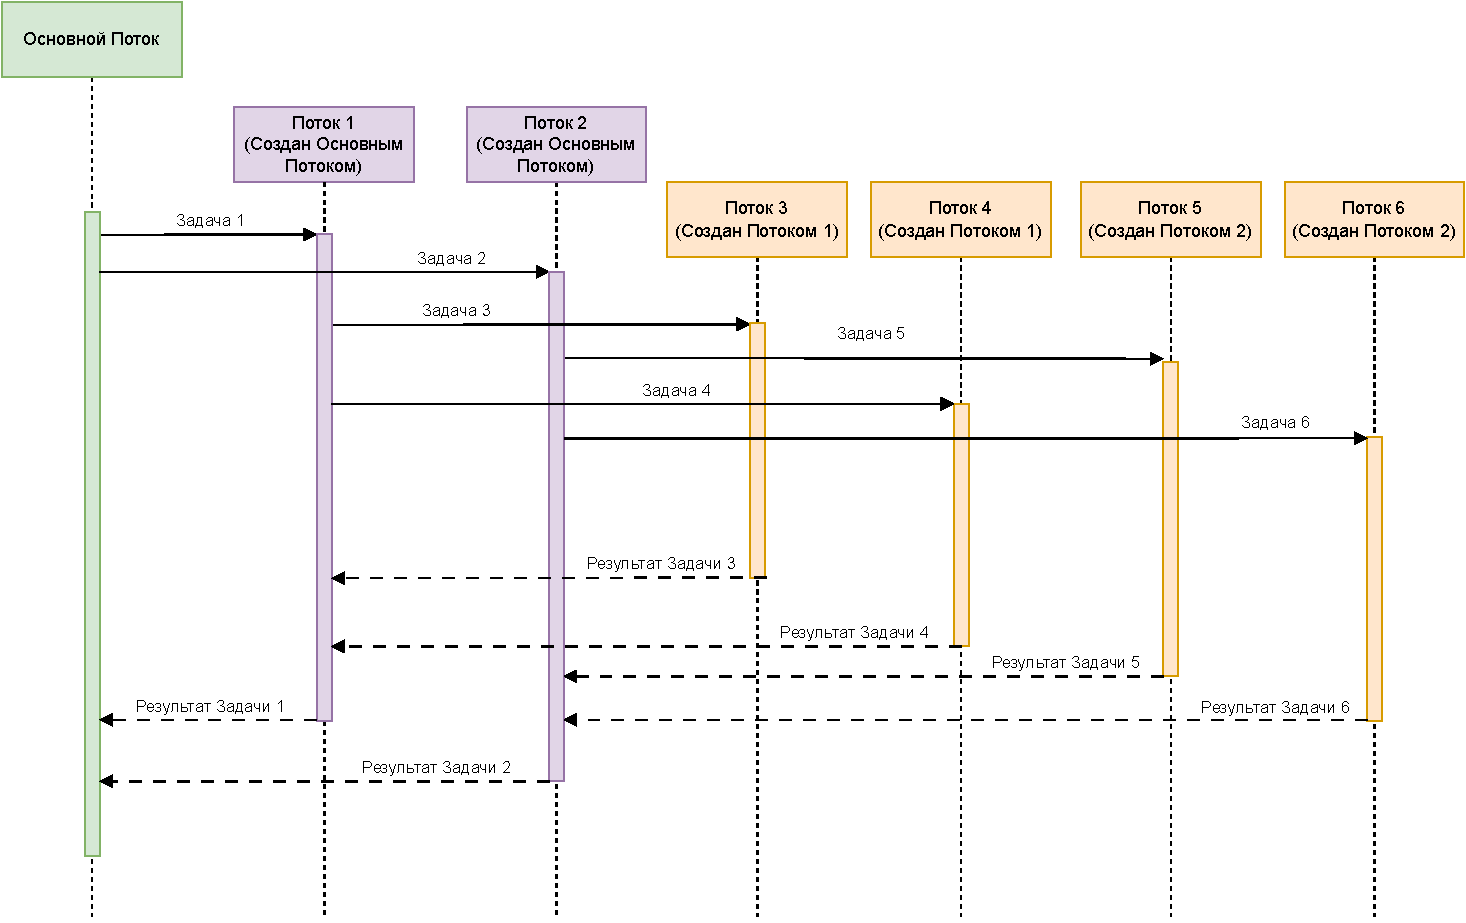
\includegraphics[width=0.9\textwidth]{SequentialUML.pdf}
    \caption{Последовательность выполнения операции сложения векторов с использованием многопоточности}
    \label{fig:uml}
\end{figure}

\subsection{Реализация BFS}

\begin{lstlisting}[style=fsharp, caption={Функция, реализующая обход в ширину с применением матрично-векторных операций.}, label={lst:bfs},  frame=single, firstnumber=32]
let BFS startVertexList (graph: Graph<'Value>) =

   let rec inner (front: Vector<unit>) visited iterationNumber =
      if front.IsEmpty then
          visited
      else
          let newFront = multiplication 0u 0u fPlus fMulti front graph.AdjacencyMatrix

          let front = vectorAddition 0u fPlusMask newFront visited

          let visited = vectorAddition 0u (fPlusVisited iterationNumber) visited front

          inner front visited (iterationNumber + 1u)

   let front = Vector(startVertexList, graph.VerticesCount, ())
   let visited = Vector(startVertexList, graph.VerticesCount, 0u)

   inner front visited 1u
\end{lstlisting}

Алгоритм BFS на листинге. \ref{lst:bfs} в точности реализует шаги 1--4, упомянутые в обзоре. Неочевидным остаётся шаг получения маски; в действительности необходимые действия выполняются в строке 40 без инициализации самой \texttt{mask}.

Функция \texttt{fPlusMask} на листинге. \ref{lst:mask} используется при сложении нового фронта и вектора посещённых вершин --- на месте \texttt{front} получается ненулевое значение, только когда вершину предстоит посетить впервые. 

\newpage

\begin{lstlisting}[style=fsharp, caption={Функция, имитирующая поведение маски для обновления вектора-фронта.}, label={lst:mask},  frame=single, firstnumber=18]
let fPlusMask a b =
    match a, b with
    | Some _, Option.None -> Some()
    | _ -> Option.None
\end{lstlisting}

